% file: sections/triangulation-one-chord.tex

\documentclass[tikz]{standalone}

\usetikzlibrary{positioning, shapes.geometric}

\begin{document}
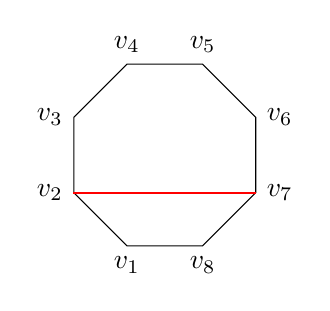
\begin{tikzpicture}
  \node (p) [draw, minimum size = 2.5cm, regular polygon, regular polygon sides = 8] {};

  \foreach \n/\cn/\pos in {1/5/below, 2/4/left, 3/3/left, 4/2/above, 5/1/above, 6/8/right, 7/7/right, 8/6/below} {
    \node (v\n) [\pos = 0.01cm of p.corner \cn] {$v_{\n}$};
  }

  \draw [red, thick] (p.corner 4) to (p.corner 7);
\end{tikzpicture}
\end{document}
